% Appendix A

\chapter{Calculating Coordinates for Line Integrals of Radon Transform} % Main appendix title

\label{AppendixA} % For referencing this appendix elsewhere, use \ref{AppendixA}

\lhead{Appendix A. \emph{Radon transform}} % This is for the header on each page - perhaps a shortened title

These minimum and maximum coordinates are calculated depends on in which of the four areas (see Figure \ref{fig:areas} ) $\theta$ resides. Because when the summation line has an absolute inclination of more than 1 will cause some pixels to be skipped.

\begin{figure}[H]
	\centering
		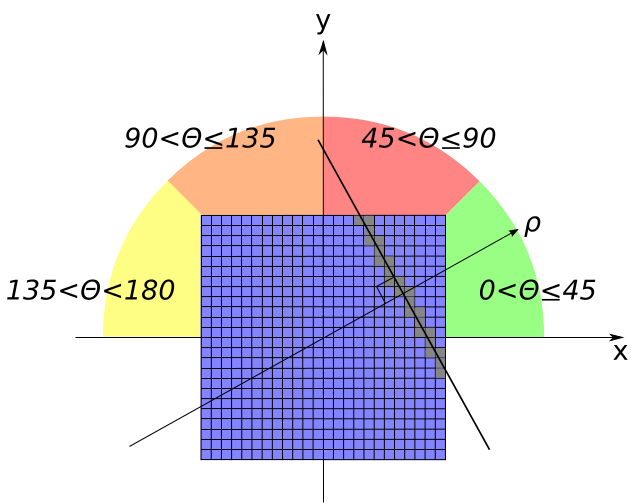
\includegraphics[width=230pt]{Figures/regions.png}
	\caption[Minimum and maximum coordinates in each region.]{Determining the maximum and minimum coordinates based on $\theta$ region.}
	\label{fig:areas}
\end{figure}


The formulas used to calculate the minimum and maximum of the variable depending on the angle $\theta$ are given below. Where $m$ is half the width of the image and $n$ is half the height of the image, $a$ is inclination, $b$ is 	the intersection with the $y$-axis and the $t_{max}$ is the size of the diagonal of the image , i.e. $t_{max}\lceil \sqrt{(2m)^2 + (2n)^2}\rceil$.
\begin{eqnarray}
0 < \theta \leq 45: \qquad  x &=& \frac{y-b}{a} \nonumber \\
	y_{min} &=& max(-n, am + b) \nonumber \\
	y_{max} &=& min(n, -am + b) \nonumber 
\end{eqnarray}

\begin{eqnarray}
45 < \theta \leq 90: \qquad  y &=& ax+b \nonumber \\
	y_{min} &=& max(-m, \frac{n-b}{a}) \nonumber \\
	y_{max} &=& min(m, \frac{-n-b}{a}) \nonumber 
\end{eqnarray}

\begin{eqnarray}
90 < \theta \leq 135: \qquad  y &=& ax+b \nonumber \\
	y_{min} &=& max(-m, \frac{-n-b}{a}) \nonumber \\
	y_{max} &=& min(m, \frac{n-b}{a}) \nonumber 
\end{eqnarray}

\begin{eqnarray}
135 < \theta \leq 180: \qquad  x &=& \frac{y-b}{a} \nonumber \\
	y_{min} &=& max(-n, -am + b) \nonumber \\
	y_{max} &=& min(n, am + b) \nonumber 
\end{eqnarray}

\begin{eqnarray}
\theta = 180: \qquad  t &=& x+ \lceil \frac{t_{max}-2m}{2} \rceil \nonumber \\
	y &=& [-m, m] \nonumber
\end{eqnarray}
